Three datasets were used for this lab:
\begin{itemize}
	\item \texttt{dataset1.txt}: 7 observations.
	\item \texttt{dataset2.txt}: 7 observations.
	\item \texttt{iris-2class.txt}: modified version of the iris dataset where classes 2 and 3 are merged such that we obtain a binary problem. 150 observations.
\end{itemize}

\textsc{Matlab} was the selected environment for this lab. In the following graphs we'll represent class 1 with a red cross \color{red}$+$ \color{black} and class -1 with a blue circle \color{blue}$\circ$\color{black}. the decision boundary will simple by a black line clearly diving both classes. \\

The hyperplane acting as the decision boundary, in this case two-dimensional, is defined by a set of parameters represented by a vector $w$. 
\begin{equation}
w = \begin{bmatrix} w_0 & w_1 & w_2 \end{bmatrix}
\end{equation}
The minimum number of parameters for representing a line in 2D space is two, however, this line will always pass through the origin. To solve this problem we introduce a bias which translates the line to any desired position in the 2D plane. The resulting hyperplane equations is:
\begin{equation}
w_0 + w_1 \, x_1 + w_2 \, x_2 = 0
\end{equation}
where
\begin{itemize}
	\item $w_0$ is the bias term.
	\item $w_1$ is the weight associated with feature $x_1$
	\item $w_2$ is the weight associated with feature $x_2$
\end{itemize}
An extra column of ones is added as an extra feature for the bias parameter, such that:
\begin{equation}
X = \begin{bmatrix} \mathbf{1} & X \end{bmatrix}
\end{equation}

\subsection{Linear classifier}
The linear classifier implemented is a rather simple one, where each observation is classified using the following:
\begin{equation}
y = \begin{cases}
-1 & \text{if} \quad X \, w^T > 0 \\
1 & \text{otherwise}
\end{cases}
\end{equation}

\subsection{Dataset 1}
The unit norm vector $w$ that \textit{best} splits the data is:
\begin{equation}
w = \begin{bmatrix}
-0.5886 & 0.4851 & 0.6468
\end{bmatrix}
\end{equation}
%
The decision boundary obtained with this $w$ is displayed in figure \ref{dataset1_1}.
\begin{figure}[h]
	\centering
	\captionsetup{justification=centering}
	\includegraphics[width=.45\textwidth]{dataset1_1}
	\caption{Dataset 1 with decision boundary.}
	\label{dataset1_1}
\end{figure}

A total of 200 random trials were carried out for every step of $p$. As norm $p$ increases, the probability of getting errors in the prediction process increases.
\begin{figure}[h]
	\centering
	\captionsetup{justification=centering}
	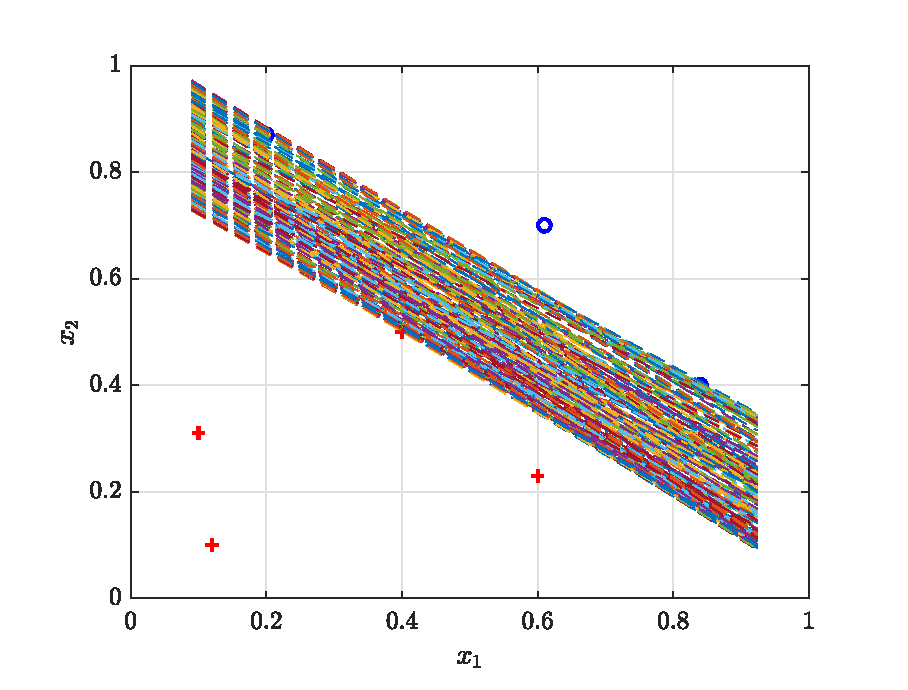
\includegraphics[width=.45\textwidth]{dataset1_2}
	\caption{Overlapped random noise with $p = 0.05$.}
	\label{dataset1_2}
\end{figure}

\subsection{Dataset 2}
The corresponding unit norm parameter vector is:
\begin{equation}
w = \begin{bmatrix}
 -0.6283  &  0.4587  &  0.6283
\end{bmatrix}
\end{equation}
%
As it can be seen from figure \ref{dataset2_1}, the observations lying on the upper-left corner of the graph are almost tangent to the decision boundary, making them prone to being misclassified when inducing noise.
\begin{figure}[h]
	\centering
	\captionsetup{justification=centering}
	\includegraphics[width=.45\textwidth]{dataset2_1}
	\caption{Dataset 2 with decision boundary.}
	\label{dataset2_1}
\end{figure}

\subsection{Iris modified dataset}
The parameter vector $w$ in unit form is:
\begin{equation}
w = \begin{bmatrix}
-0.2408  &  -0.1204  &  0.9631
\end{bmatrix}
\end{equation}
%
\begin{figure}[h]
	\centering
	\captionsetup{justification=centering}
	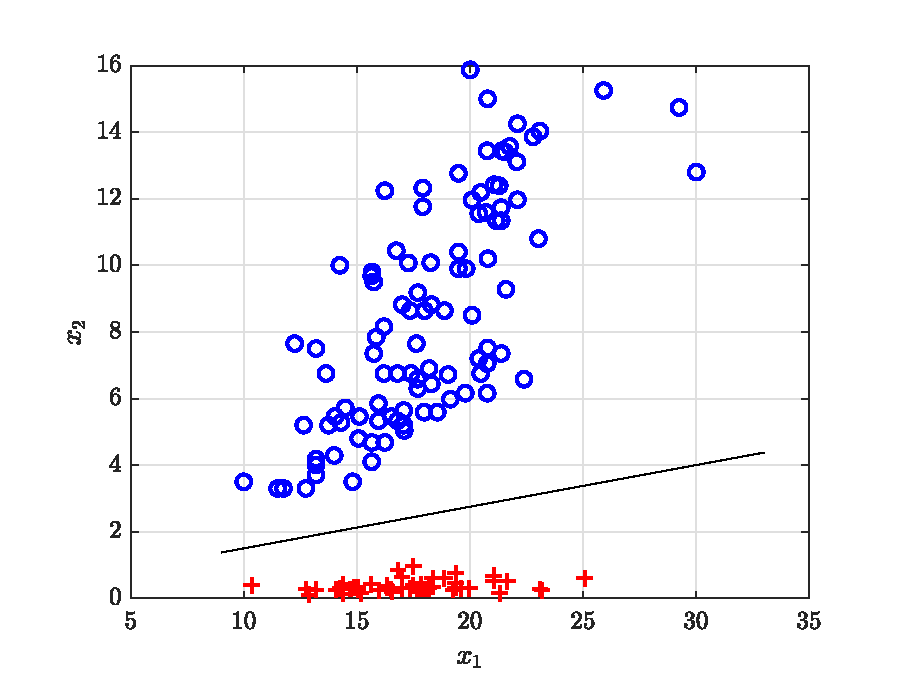
\includegraphics[width=.45\textwidth]{dataset3_1}
	\caption{Iris modified dataset with decision boundary.}
	\label{dataset3_1}
\end{figure}

An interesting behavior is observed when adding noise. In contrast with the previous datasets, the feature range in the iris dataset allows us to realize that the noise acquires a conic shape. Points lying far from the origin will be more sensitive to noise than those lying closer. Curiously enough, the observations seem to follow this conic shape but it won't always be like this.
\begin{figure}[h]
	\centering
	\captionsetup{justification=centering}
	\includegraphics[width=.45\textwidth]{dataset3_2}
	\caption{Conic shaped random noise with $p = 0.1$.}
	\label{dataset3_2}
\end{figure}
